% This is samplepaper.tex, a sample chapter demonstrating the
% LLNCS macro package for Springer Computer Science proceedings;
% Version 2.20 of 2017/10/04
%
\documentclass[runningheads]{llncs}
%
\usepackage{graphicx}
%\usepackage{ngerman}
\usepackage[utf8x]{inputenc}
\usepackage{fancyvrb}
\usepackage{courier}
\usepackage{helvet}
\usepackage{tikz}
\usepackage{xcolor}
\usepackage{pdfpages}
\usetikzlibrary{calc}
\usepackage[strict]{changepage}
\usepackage{xspace}
\usepackage{hyperref}
\usetikzlibrary{shapes.geometric}
\usetikzlibrary{arrows}
\usetikzlibrary{positioning}
\usetikzlibrary{arrows.meta, automata, shapes, matrix,positioning}
\usepackage{amssymb}
\usepackage{pifont}% http://ctan.org/pkg/pifont
\usepackage{subcaption} 
\usepackage{float}
\usepackage{fixfoot}
\usepackage{graphicx}
\usepackage{wrapfig}
\usepackage{multicol}
\usepackage{amsmath}
\usepackage{cleveref}
\usepackage{listings}

\newcommand{\cmark}{\ding{51}}%
\newcommand{\xmark}{\ding{55}}%
% Used for displaying a sample figure. If possible, figure files should
% be included in EPS format.
%
% If you use the hyperref package, please uncomment the following line
% to display URLs in blue roman font according to Springer's eBook style:
% \renewcommand\UrlFont{\color{blue}\rmfamily}

\begin{document}
	%
	\title{Clustering Analysis of Mobility Data}
	%
	%\titlerunning{Abbreviated paper title}
	% If the paper title is too long for the running head, you can set
	% an abbreviated paper title here
	%
	\author{Miriam Wagner\and
		Martin Breuer\and
		Moritz Werthebach\and
		Timo Bergerbusch\and
		Walter Schikowski}
	%
	\authorrunning{F. Author et al.} %TODO
	% First names are abbreviated in the running head.
	% If there are more than two authors, 'et al.' is used.
	%
	\institute{RWTH Aachen, Templergraben 55, 52062 Aachen, Germany}
	%
	\maketitle              % typeset the header of the contribution
	%
	\begin{abstract} %TODO
		The abstract should briefly summarize the contents of the paper in
		150--250 words.
		
		\keywords{Clustering \and Rapidminer \and Cluster \and Data Mining} %TODO: maybe more
	\end{abstract}
	%
	%
	%
	\section{Introduction}
	\section{Preprocessing}\label{sec: proprocessing}
	In order to classify the given data into smaller test sets or mask different aspects, we have to perform analysis.\\
	We observe that even though we have 124979 individual lines defining a movement, there is one line defining a \texttt{NotANumber}-exception and therefore gets neglected for further usage.	\\
	We provide the \texttt{testDataGenerator} python script. Through flags and input arguments the script is able to create all test sets considered by our clustering and neural net approaches.\\
	%TODO: should this be within the paper or more in a ReadMe-file delivered with the script itself?
%	The possible flags and an explanation can be taken from \Cref{fig: testdatagenerator flags}.	
%	\begin{figure}[H]
%		\centering
%		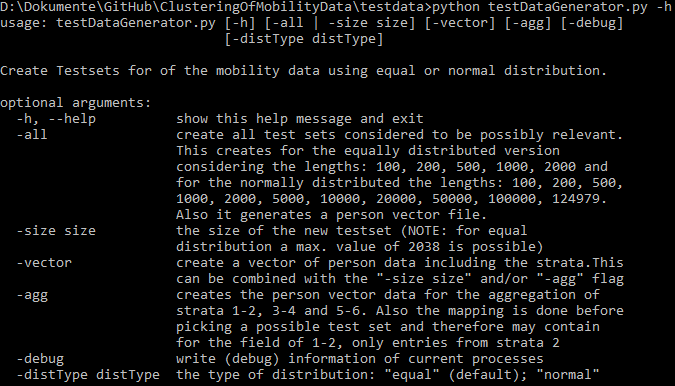
\includegraphics[scale=0.5]{src/pic/testDataGenerator-h.PNG}
%		\caption{The possible arguments to the \texttt{testDataGenerator}}
%		\label{fig: testdatagenerator flags}
%	\end{figure}
	We observe the following distribution over the whole dataset:\\
	{\hspace*{2cm}\setlength\tabcolsep{.2cm}\begin{tabular}{c|ccccccc}
		strata &  1   &   2   &   3   &  4   &  5   &  6   & $\Sigma$ \\ \hline
		 abs   & 6963 & 52265 & 49404 & 8772 & 5536 & 2038 &  124978  \\
		  \%   & 5.57 & 41.82 & 39.53 & 7.02 & 4.43 & 1.63 &   100
	\end{tabular}}\\
	We observe that there is an upper bound on equal distribution through strata 6. It has at most 2038 individual elements.
	
	In addition to the original paper we compute the value \texttt{ID}, which is used to combine movements considered to be from the same person.
	We consider two movements to coincide on the underlying person, if and only if they are consecutive in the original dataset and have the same strata, age and gender.
	{\hspace*{2cm}\setlength\tabcolsep{.2cm}\begin{tabular}{c|ccccccc}
		strata &  1   &   2   &   3   &  4   &  5   &  6  & $\Sigma$ \\ \hline
		 abs   & 3153 & 23367 & 21418 & 3497 & 2083 & 595 &  54113   \\
		  \%   & 5.83 & 43.18 & 39.58 & 6.46 & 3.85 & 1.1 &   100
	\end{tabular}}\\
	So we also have through strata 6 an upper bound of 595 for equally distributed person vector data (see \Cref{subsec: person vector data}).
	
	\subsection{Vector}\label{subsec: person vector data}
	As stated before, instead of simple IDs for every person we expand the parsing by using a data encapsulating in a class called \texttt{Person}. This class stores the ID, the parameters defining a person %TODO: ref zu code basics
	, and all movements from that person.\\
	Then we are able to compute the following vector, with 848 entries, for further usage, that combines all movements of the person:
	\begin{align*}
	\underbrace{\#o_1, \dots, \#o_{413}, \#d_1, \dots, \#d_{413}}_{2\cdot 413} ,
	\underbrace{\mathit{AM}, \mathit{MD}, \mathit{PM}, \mathit{MN}}_{4}, 
	\underbrace{\#r_1, \dots, \#r_7}_{7}, \\
	\underbrace{\#\mathit{MoT}_1, \dots, \#\mathit{MoT}_7}_{7}, \underbrace{\mathit{SDest}, \mathit{SDist}, \mathit{G}, \mathit{A} ,\mathit{strata}, \mathit{strataGrouped}}_{6}
	\end{align*}
	with the following abbreviations ($1 \le i \le 413$, $1 \le j \le 7$):
	\begin{multicols}{2}
		\begin{itemize}
			\setlength{\itemindent}{.4cm}
			\item[$o_i$:]  the $i$-th origin data point
			\item[$d_i$:]  the $i$-th destination data point
			\item[$\mathit{AM}$:] movements at time stamp AM
			\item[$\mathit{MD}$:] movements at time stamp MD
			\item[$\mathit{PM}$:] movements at time stamp PM
			\item[$\mathit{MN}$:] movements at time stamp MN
			\item[$r_j$:] the $j$-th reason
			\item[$\mathit{MoT}_j$:] the $j$-th mean of transportation
			\item[$\mathit{SDest}$:] sum of all durations
			\item[$\mathit{SDist}$:] sum of all distances
			\item[$\mathit{G}$:] the gender
			\item[$\mathit{A}$:] the age
			\item[$strata$:] the strata (used for comparison)
			\item[$strataGrouped$:] the aggregated stratas
		\end{itemize}
	\end{multicols}
	\section{Predicting}
	
	\subsection{Classification}
%	%Miriam Clustering
\setlength{\parindent}{0em}
The first question was: is it possible without knowing the social classes to reproduce them based on the movement data. Therefore we wanted to look for clusters and compare those with the strata. Also we had a look if the possibly found clusters have special properties.

\subsubsection{Clustering with RapidMiner}

RapidMiner has different Modules for Clustering already implemented. We decided to concentrate on the k-means clustering algorithm.
\begin{figure}[!htbp]
\centering
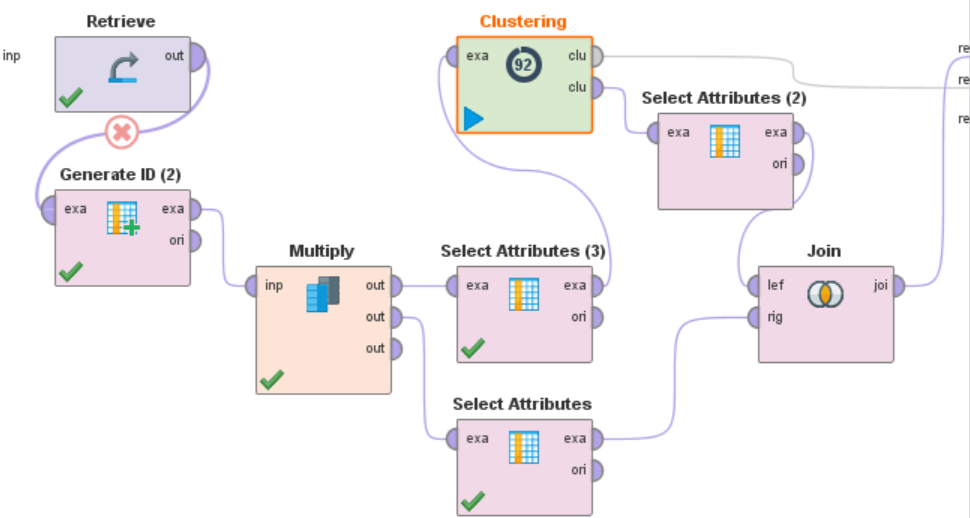
\includegraphics[width=0.9\textwidth]{ClusteringRapid.PNG}
\caption{Process of k-means clustering}
\label{fig: kclust}
\end{figure}


The Process, figure \ref{fig: kclust}, contains the following steps:
\begin{description}
	\item[Retrieve] gives the data into the process. 
  \item[Generate ID] creates an ID such that we can make the comparsion step at the end through joining the sets
  \item[Multiply] creates two identical data sets
  \item[Select Attrbiutes] thoughs away the strata before the clustering step, everything behalve cluster and id after the clustering and just keeps id and strata for the join step
	\item[Clustering] runs the k-means clustering algorithm. The number of Clusters has to be fixed.
	\item[Join] For comparing the clustering result and the strata we join the two filtered data sets by the id
\end{description}

In the clustering block we can chose between different distance measures and maximal step numbers. We decided to concentrate on almost everywhere basic configurations and chose the squared euclidean distance in the mixed version.

In the first step we tried to cluster the \textbf{Original Data} in \textbf{6 Cluster}. Therefore we retrieved the original data set in RapidMiner and chose k as 6.

\ref{fig:OrgDist}. 
\begin{figure}[!htbp]
\centering
\begin{subfigure}{.5\textwidth}
  \centering
  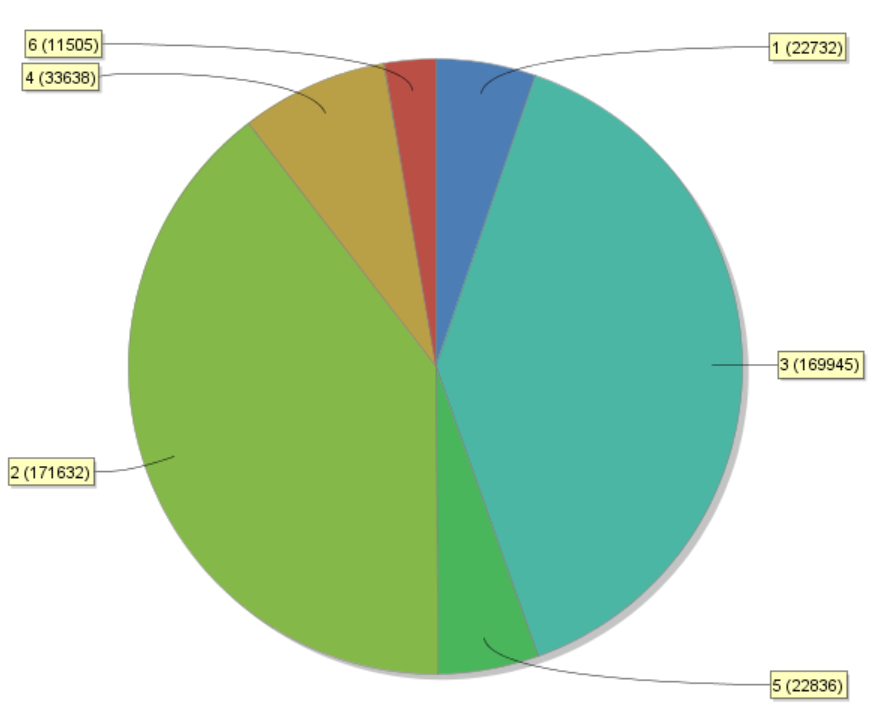
\includegraphics[width=.8\linewidth]{ClusterOrigRapidStrata.PNG}
  \caption{Strata}
  \label{fig:OrgSt}
\end{subfigure}%
\begin{subfigure}{.5\textwidth}
  \centering
  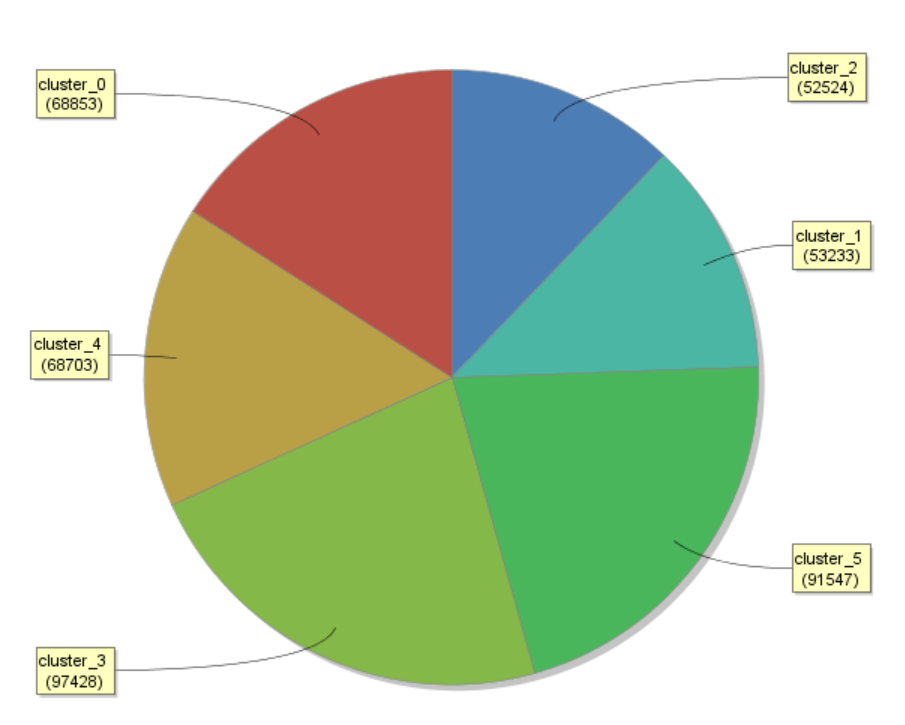
\includegraphics[width=.8\linewidth]{ClusterOrigRapidCluster.PNG}
  \caption{Cluster}
  \label{fig:OrgCl}
\end{subfigure}
\caption{Distribution of original data}
\label{fig:OrgDist}
\end{figure}

In figure \ref{fig:OrgDist} is the result to see of the first try. Figure \ref{fig:OrgSt} shows the strata distribution as pie chart and \ref{fig:OrgCl} the resulted cluster distribution. It can already been seen, that the distributions are not similar. In the next step we tried it with more steps, but the result was not looking better.

We asked ourselfs, if 6 cluster is not too fine, so we searched for \textbf{3 clusters} in the next step. The idea is to combine two stratas in 1, such that we just have 3 stratas left.
\begin{figure}[!htbp]
\centering
\begin{subfigure}{.5\textwidth}
  \centering
  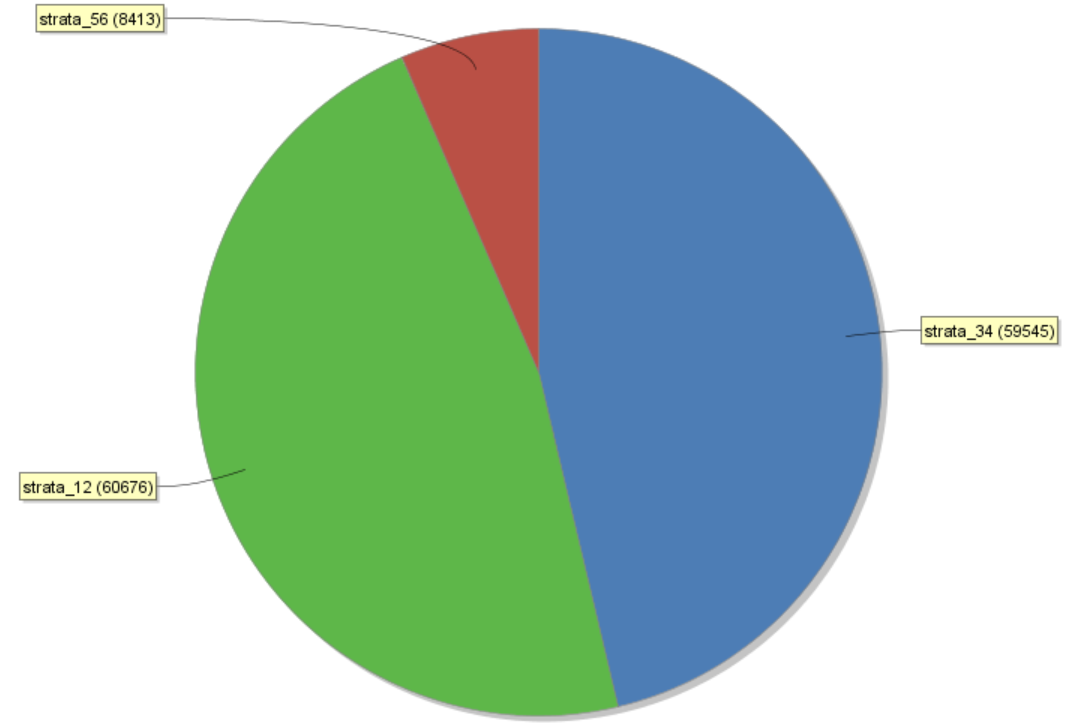
\includegraphics[width=.8\linewidth]{ClusterOrigRapidStrata2Cluster.PNG}
  \caption{Strata}
  \label{fig:OrgSt}
\end{subfigure}%
\begin{subfigure}{.5\textwidth}
  \centering
  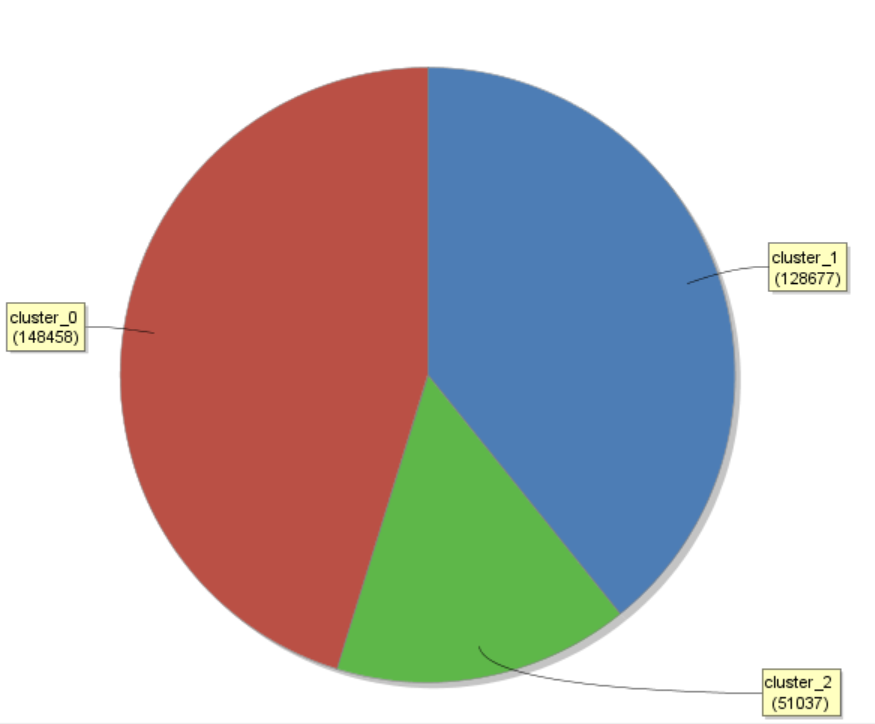
\includegraphics[width=.8\linewidth]{ClusterOrigRapidCluster2Cluster.PNG}
  \caption{Cluster}
  \label{fig:OrgCl}
\end{subfigure}
\caption{Distribution of original data for just 3 clusters}
\label{fig:OrgDist3Cl}
\end{figure}

\begin{figure}[!htbp]
\centering
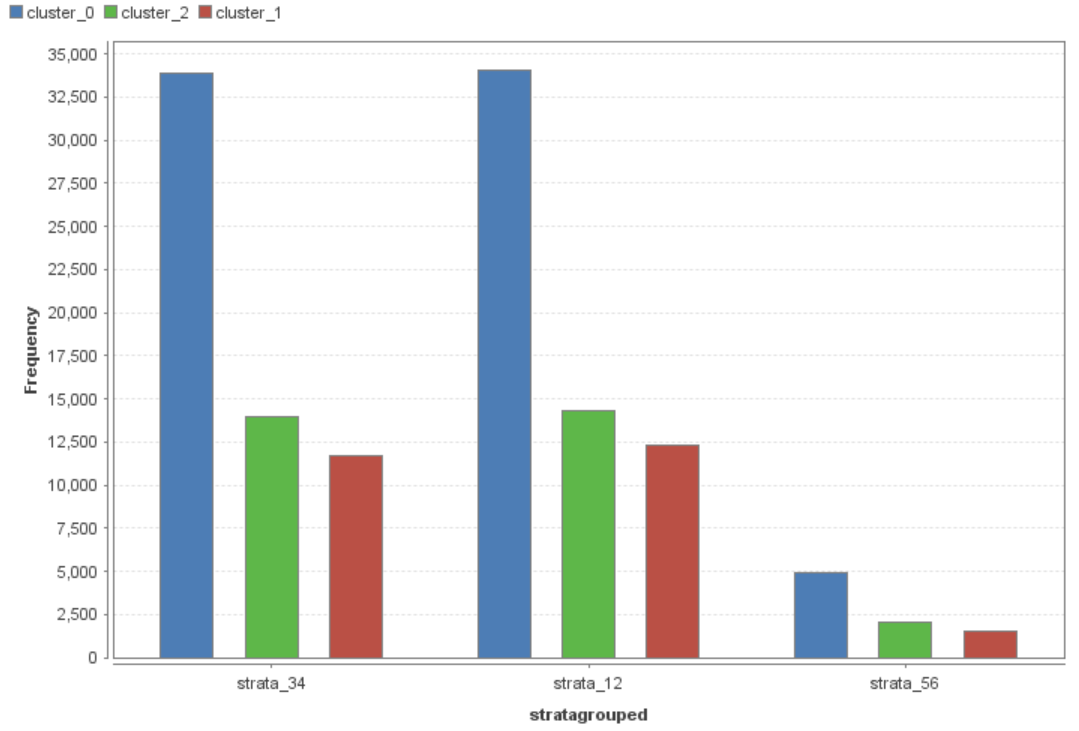
\includegraphics[width=0.9\textwidth]{ClusterOrigRapidDistribution2Cluster.PNG}
\caption{Distribution of the clusters in between the grouped strata}
\label{fig:Groupdist}
\end{figure}

After having a look at the pie charts, \ref{fig:OrgDist3Cl} and so the distribution in between the variable it seems to be a better result, so we had a look at the cluster distribution in the 3 grouped stratas, \ref{fig:Groupdist}. This figure shows clearly, that there is no real correlation between strata 

\begin{figure}[!htbp]
\centering
\begin{subfigure}{0.9\textwidth}
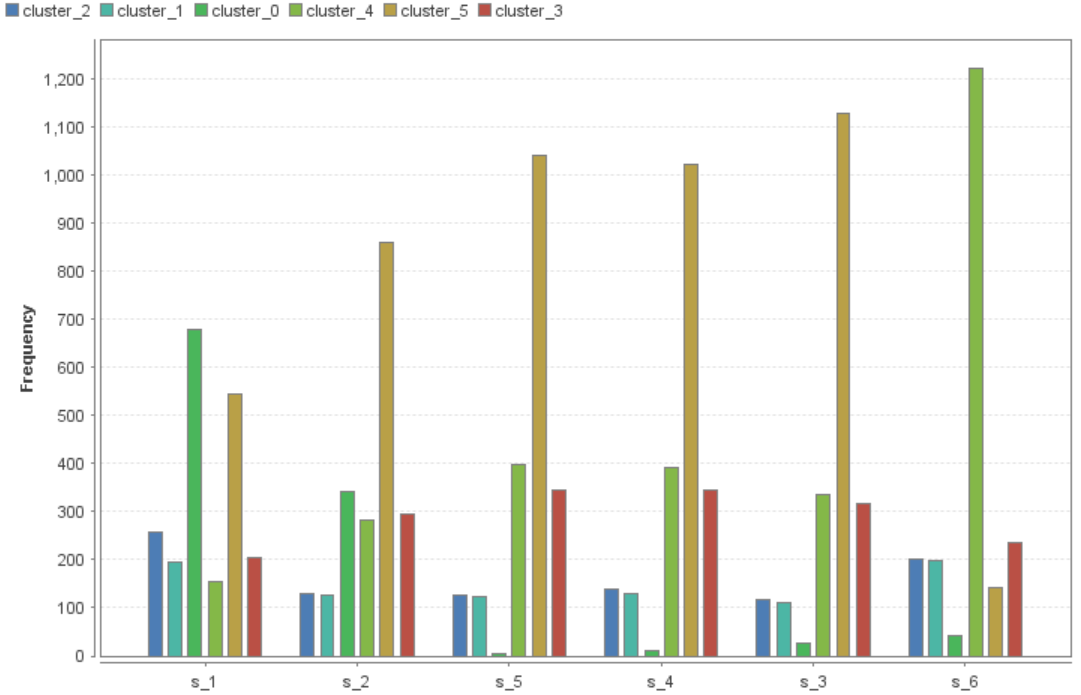
\includegraphics[width=\linewidth]{ClusterOrigRapidDistribution2038eq.PNG}
\caption{For 6 clusters}
\label{fig:2038_6}
\end{subfigure}
\begin{subfigure}{0.9\textwidth}
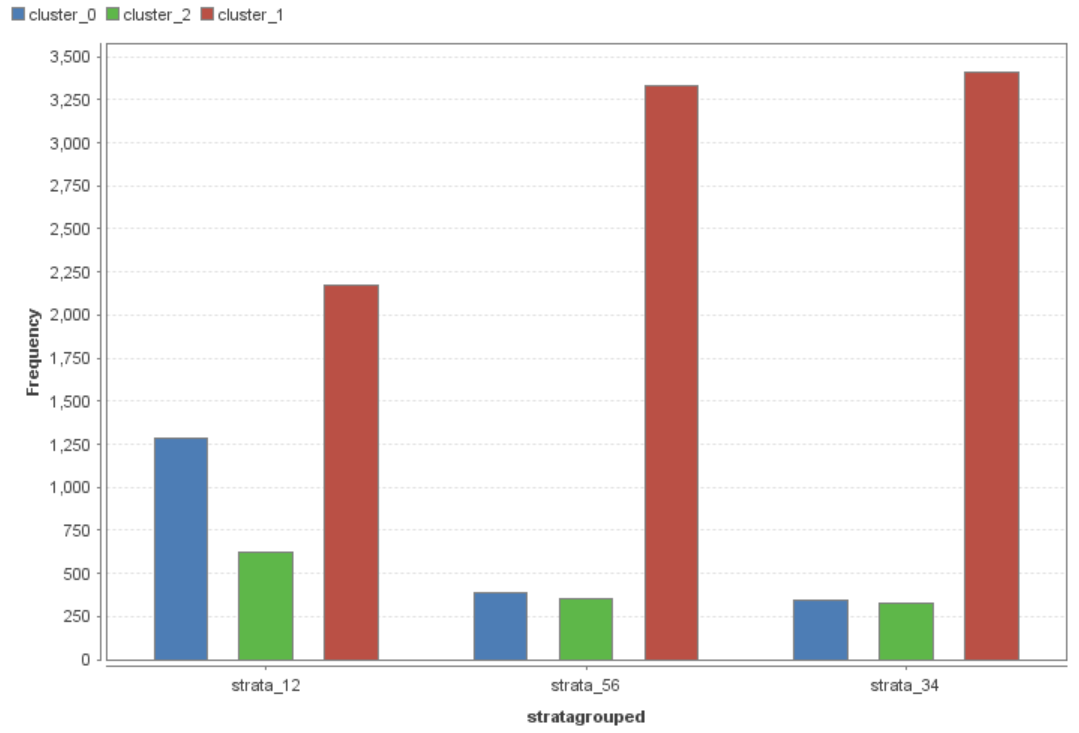
\includegraphics[width=\linewidth]{ClusterOrigRapidDistribution2038eq2.PNG}
\caption{For 3 clusters}
\label{fig:2038_3}
\end{subfigure}
\caption{Distribution of the clusters in between the strata}
\label{fig:2038_Clust}
\end{figure}

The result for different datasizes and equal distribution of the stratas does not change the result. The biggest equal distributed dataset has 2038 data rows for every strata and 4076 in between the grouped strata. In figure \ref{fig:2038_Clust} the two clustering results can be seen. Again we could not really see a significant correlation.

\textbf{Stratified Person Data}

After those not really convincing results we applied the process on the stratified person data, because those represented the movement of one person.

\begin{figure}[h]
\centering
\begin{subfigure}{.5\textwidth}
  \centering
  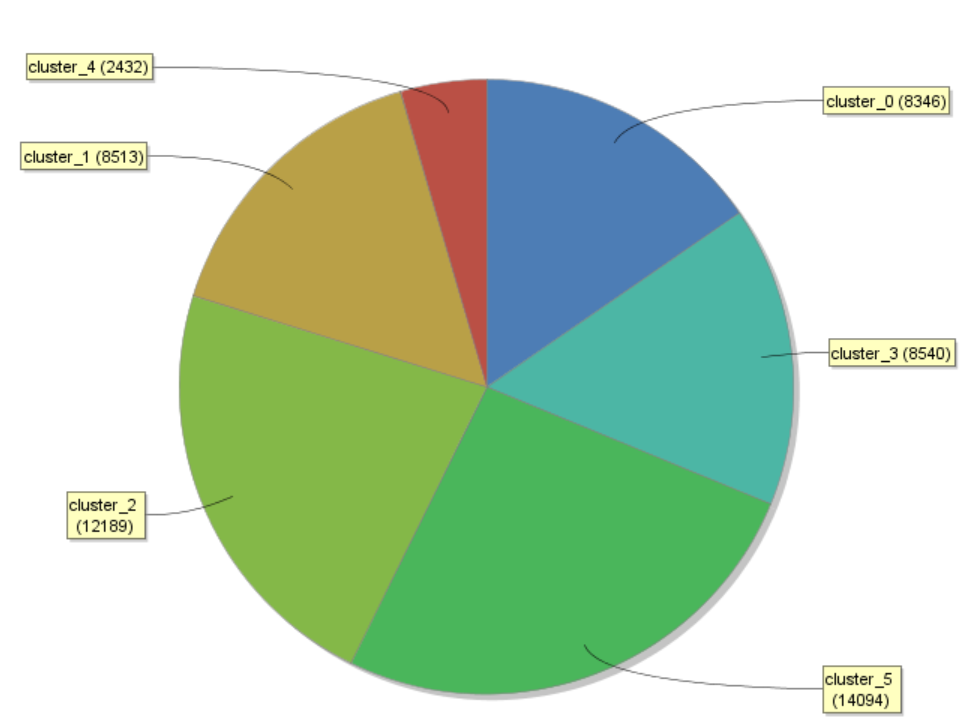
\includegraphics[width=.9\linewidth]{vectorclusteringcluster.PNG}
  \caption{Strata}
  \label{fig:VecSt}
\end{subfigure}%
\begin{subfigure}{.5\textwidth}
  \centering
  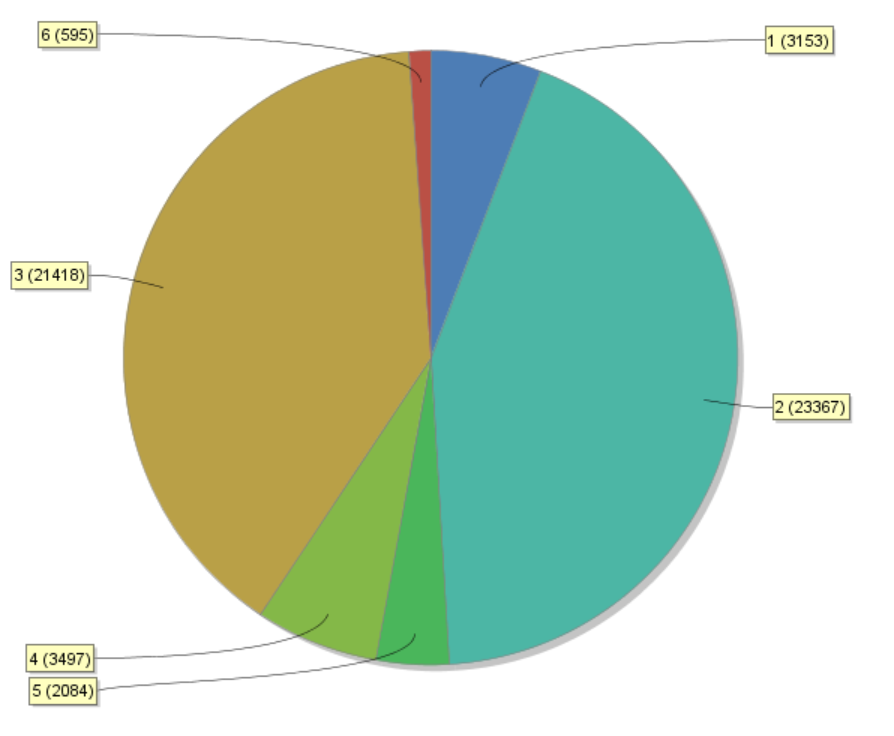
\includegraphics[width=.9\linewidth]{vectorclusteringstrata.PNG}
  \caption{Cluster}
  \label{fig:VecCl}
\end{subfigure}
\caption{Distribution of stratified person data}
\label{fig:VecDist}
\end{figure}

\begin{figure}[!htbp]
\centering
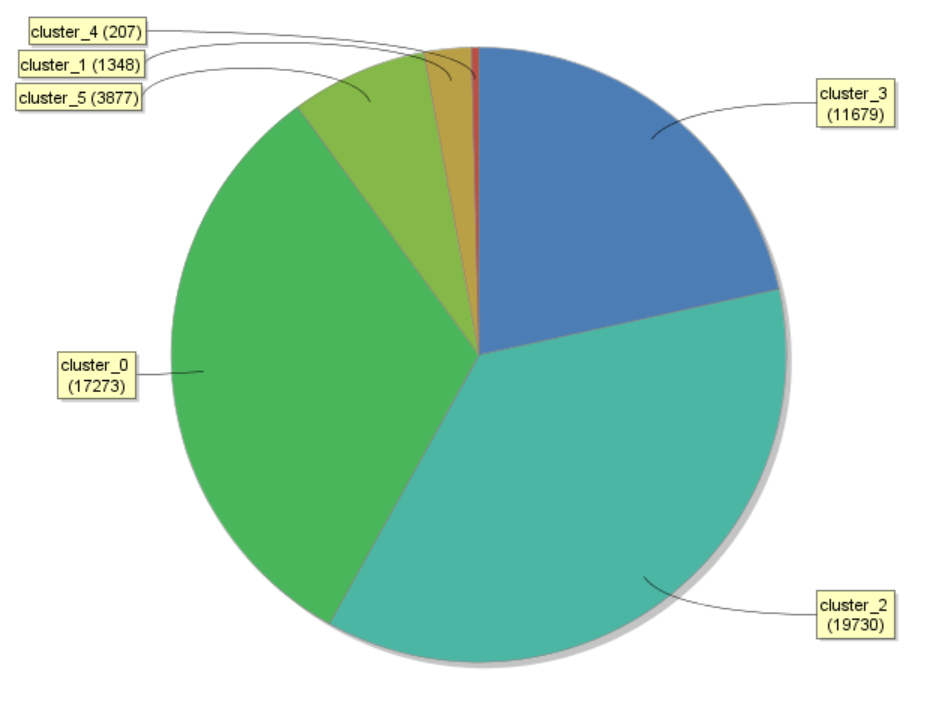
\includegraphics[width=0.3\textwidth]{vectorclusteringcluster1000.PNG}
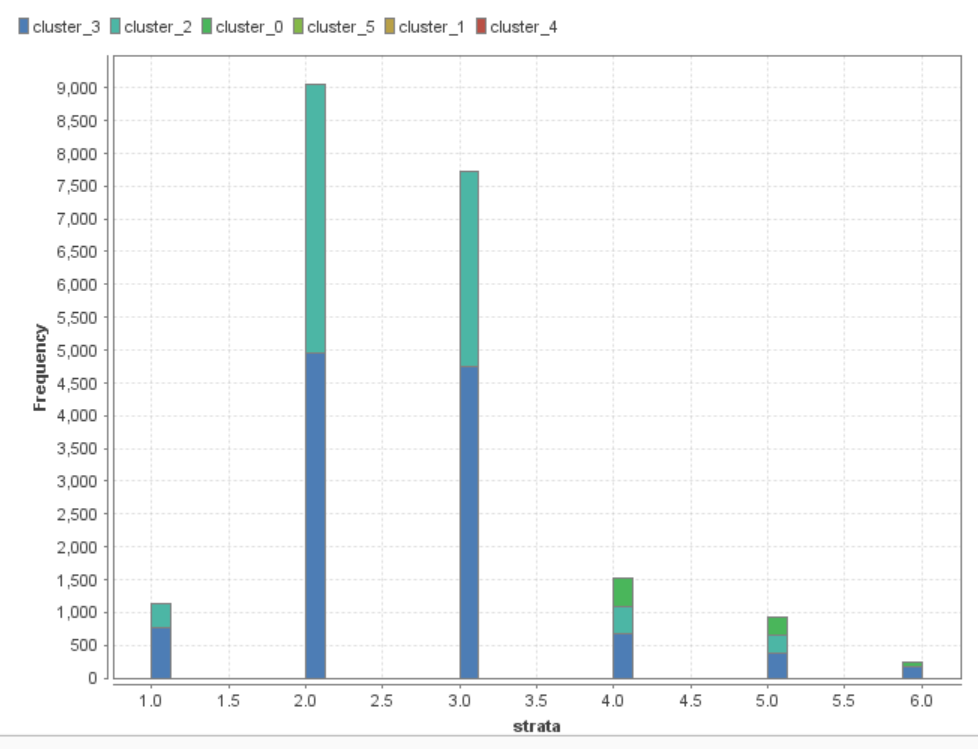
\includegraphics[width=0.69\textwidth]{vectorClustering1000.PNG}
\caption{1000 steps clustering in 6 clusters}
\label{fig:1000vect}
\end{figure}

The results for the whole data set without equalization are shown in figure \ref{fig:2038_Clust}. We changed the number of steps to 1000 for comparsion and the result, \ref{fig:1000vect}, let us assume, that 3 clusters better would fit. 


So we applied the process on the \textbf{stratified person data} and searched for \textbf{3 clusters}. We directly run the algorithm 1000 steps.

\begin{figure}[!htbp]
\centering
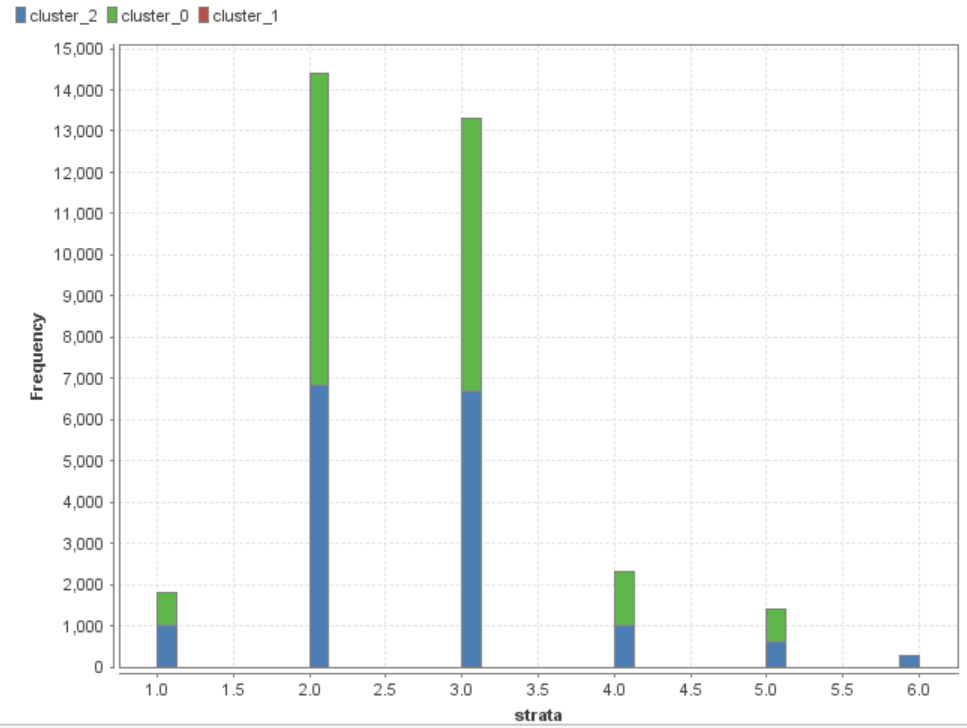
\includegraphics[width=0.69\textwidth]{vectorClustering31000.PNG}
\caption{1000 steps clustering in 3 clusters}
\label{fig:1000vect3}
\end{figure}

Figure \ref{fig:1000vect3} shows clearly, that again no correlation can be found. Furthermore we applied this for the different datasets we generated, but the result was always similar.


%PCA??
	\subsection{Neural Net}
	For all the neural net computations we considered person vector data sets of different sizes (c.f. \Cref{subsec: person vector data}).\\
	
	We do this, because results on the normal datasets had an unacceptable performance, since only single movements and not complete paths of individuals are considered. An example training and performance measure is given in \Cref{fig: NN without vector} where unprocessed data is used. The performance is measured using 10-fold cross validation, i. e. the data is split into 10 subsets where in each iteration exactly one data set is used as test set and the other 9 as training set. The average value of the accuracy values lead
	 to the total accuracy value of the neural net.
	\begin{figure}[H]
		\centering
		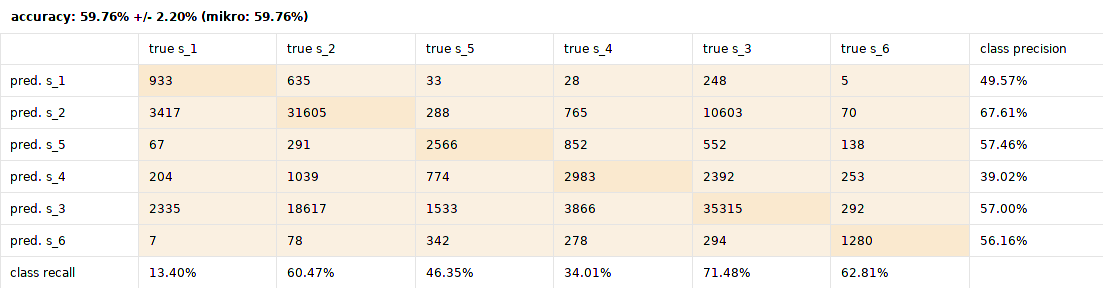
\includegraphics[scale = 0.4]{src/pic/NN_without_vector.png}
		\caption{An example of a neural net trained without person vector data.}
		\label{fig: NN without vector}
	\end{figure}
	
	In the following we consider 3 neural nets $\mathcal{N}_1,\mathcal{N}_2$ and $\mathcal{N}_3$, all having 4 hidden layers, 50 epochs and 10 iterations.	
	As an example of other strata aggregation we combine the stratas 1--2, 3--4 and 5--6 together and call them $\mathcal{N}_i^\star$, for $i \in \{5,10,20\}$. This builds a superset of the original stratas and since the stratas themselves are logically connected this task should be easier to fulfill.\\
	
	For each neural net we are using equally distributed data sets with 100, 200 and the maximal amount of 595 individuals per strata which are provided by the \texttt{testDataGenerator} from \Cref{sec: proprocessing}. For every neural net and every set size we performed 5 independent runs and calculated the average over those accuracy values in order to have a sophisticated, comparable statements. 
	\setlength\tabcolsep{.2cm}
	\begin{figure}[H]
	\centering
	\begin{tabular}{|c|c|c|c|c|c|}
		\hline
		                         &   \#    &        & \multicolumn{3}{c|}{Set size} \\
		          Name           & Neurons &   AG   &  100  &  200  &      595      \\ \hline
		    $\mathcal{N}_5$      &    5    & \xmark & 60.03 & 59.92 &     60.18     \\
		 $\mathcal{N}_5^\star$   &    5    & \cmark & 87.6  & 89.7  &     71.05     \\
		   $\mathcal{N}_{10}$    &   10    & \xmark & 75.83 & 73.54 &     69.56     \\
		$\mathcal{N}_{10}^\star$ &   10    & \cmark & 92.93 & 93.48 &     74.58     \\		
		%		$\mathcal{N}_{10}^\star$ &   10    & \cmark & 88.33 {\small $\pm$7.49} & 90.67{\small $\pm$2.81} & 92.14 {\small $\pm$ 2.59} \\
		   $\mathcal{N}_{20}$    &   20    & \xmark & 75.45 & 71.14 &     61.87     \\
		$\mathcal{N}_{20}^\star$ &   20    & \cmark & 92.87 & 94.4  &     78.32     \\ \hline
	\end{tabular}
	\caption{The accuracy values of the neural nets. (See excel-spreadsheet)}
	\label{tab: nn-accuracy}
	% mittels deep-learning-vector-average
	\end{figure}


	The size of larger nets in terms of neurons is counter-productive, since if we take 50 neurons per layer we have $14 \cdot 50^4 \cdot 6 \approxeq 525.000.000$ synapses for which the input data set would be to small to have sufficient training.\\

	%TODO: what can we oberve?
%	The greater the population, the more the borders between the stratas blur. 



\end{document}
